This section will introduce the field of Quantum Computing, the theories and concepts and some algorithms, leading up to an adaptation of Shor's algorithm for discrete logarithms of elliptic and hyperelliptic curves.
\subsection{Properties of Quantum Computers}
\subsubsection{Qubits}
To begin to describe quantum computing, we can start at the very basis of the concept. The basis of a classical computer is a bit, which is usually stored in a transistor which can either have a voltage or not, i.e. the bit holds either a 1 or a 0. In a similar way, we can define the notion of a \emph{qubit}, the equivalent to a classical bit, and how it is physically implemented. Many particles and atoms posess a quality called "magnetic spin", which means that they can be deflected under a magnetic field. A particle's spin can either be up spin or down spin, meaning that the particle will either be deflected up or down when subject to a magnetic field, particles will never be deflected to the side or any other direction. Until we measure this spin property, the particle exists in a "superposition" of both up and down spin, and we have no way of predicting which type of spin the particle will have. Once the spin of the particle is measured, then this superposition collapses and the particle behaves in a non quantum way. A way of representing this spin is to assign a probability to each state as such: $$\ket{\psi} = \alpha_0\ket{0} + \alpha_1\ket{1}$$ Where $\ket{\psi}$ represents the superposition of the particle, $\alpha_0\ket{0}$ represents the probability $\alpha_0$ of the particle having up spin $\ket{0}$, and $\alpha_1\ket{1}$ represents the probability of the particle having down spin. The notation $\ket{0}$ is known as \emph{ket} notation, and is used frequently when describing quantum computing. This superposition then becomes our qubit, on which we can perform various operations to affect the output value, and the building block from which we can build a quantum system.
\subsubsection{Quantum States}
A classical system with n components, each of which can have two states (1 or 0) can be represented in full by n bits. A quantum system with n qubits would require $2^{n}$ complex number coefficients, or more precisely, the state of the quantum computer can be thought of as a point in a $2^{n}$-dimensional vector space, and for each of these $2^{n}$ states, we can represent them as a probability multiplied by a basis state, for example: $\alpha_i\ket{0010}$ means that the probability of the system being in state $\ket{0010}$ is equal to $\alpha_i$. The state of the whole system at any time can be represented by a \emph{Hilbert space} defined as:
$$ \ket{\psi} = \alpha_0\ket{\phi_0} + \alpha_1\ket{\phi_1} + ... + \alpha_{2n-1}\ket{\phi_{2n-1}} = \sum_{i=0}^{2^{n}-1} \alpha_{i} \ket{\phi_i} $$
where the amplitudes $a$ are complex numbers such that $\sum_{i}|\alpha_{i}|^{2} = 1$, and each $\ket{\phi_i}$ is a basis vector of the Hilbert space. The probability of the machine being at a basis state $\ket{\phi_i}$ at any time is $|\alpha_i|^2$, however reading the machines state at any time will invalidate the rest of the computation since this state will then be projected to the observed basis vector $\ket{\phi_i}$. For an example of this, suppose we have the quantum state: $\ket{\psi} = \frac{1}{\sqrt{3}}\ket{0} + \sqrt{\frac{2}{3}}\ket{1}$, then the probability of measuring the basis state $\ket{0}$ is equal to $\frac{1}{\sqrt{3}}^2 = \frac{1}{3}$, and the probability of measuring the basis state $\ket{1}$ is equal to $\sqrt{\frac{2}{3}}^2 = \frac{2}{3}$. We also have the \emph{conjugate} state, which can be represented in \emph{bra} notation: $\bra{\psi}$. If we have the quantum state $\ket{\psi} = \sum_i\alpha_i\ket{\phi_i}$, then the conjugate state is: $\bra{\psi} = \sum_i\alpha_i^*\bra{\phi_i} = \begin{pmatrix} \alpha_0^* & \alpha_1^* & ... & \alpha_{2n-1}^* \end{pmatrix}$ i.e. a row vector of the \emph{complex conjugates} of the elements of $\ket{\psi}$ with the complex conjugate of a complex number $a + b\textit{i}$ being $a -b\textit{i}$.
\subsubsection{Transformations on Quantum States}
Machine states can be described in vector format by taking all the coefficients as such: $$\ket{\psi} = \alpha_0\ket{\phi_0} + \alpha_1\ket{\phi_1} \equiv \begin{pmatrix} \alpha_0 \\ \alpha_1 \end{pmatrix}$$ We can then apply a transformation to this state such that the coefficients become $\alpha_0'$ and $\alpha_1'$: $$\ket{\psi'} = \alpha_0'\ket{\phi_0} + \alpha_1'\ket{\phi_1} \equiv \begin{pmatrix} \alpha_0' \\ \alpha_1' \end{pmatrix}$$ This transformation can be expressed as $$\ket{\psi'} = U\ket{\psi}$$ where $U$ is a unitary $m\times m$ matrix with $m$ being the size of the state, which in our case is 2. Therefore, our transformation can be represented as: $$\begin{pmatrix} \alpha_0' \\ \alpha_1' \end{pmatrix} = \begin{pmatrix} u_{11} & u_{12} \\ u_{21} & u_{22} \end{pmatrix} \begin{pmatrix} \alpha_0 \\ \alpha_1 \end{pmatrix},$$ and we have that $\alpha_0' = u_{11}\alpha_0 + u_{12}\alpha_1$ and $\alpha_1' = u_{21}\alpha_0 + u_{22}\alpha_1$
\subsubsection{Bell States and Entanglement}
Bell states are quantum states where qubits are entangled, i.e. if we measure one of the qubits, we know what the other one will be without having to measure it. An example of such a state is: $$\ket{\psi} = \frac{\ket{00} + \ket{11}}{\sqrt{2}}$$
Entangled states cannot be created from independent qubits, instead they have to be programmed using quantum circuits. Consider the composite state: $$a_0b_0\ket{00} + a_0b_1\ket{01} + a_1b_0\ket{10} + a_1b_1\ket{11},$$ composed of two independent qubits: $a_0\ket{0} + a_1\ket{1}$ and $b_0\ket{0} + b_1\ket{1}$. For this to be a bell state, we require the only possible states when measured to be $\ket{00}$ and $\ket{11}$, therefore $a_0b_1$ and $a_1b_0$ both have to equal 0, however this leads to a contradiction in classical mechanics, because whichever configuration we choose for $a_0b_1$ and $a_1b_0$ to equal 0, means that $a_1b_1$ and $a_0b_0$ are also equal to 0, but in reality, these are equal to $\frac{1}{\sqrt{2}}$. This is where the properties of quantum mechanics start to differ from classical mechanics. Entanglement is what makes quantum computers truly powerful, as otherwise, the same computation can be simulated on classical computers. Creating entangled qubits is very hard to do however, and at time of writing, the largest number of entangled qubits in a physical quantum computer is 20~\cite{mooney2019entanglement}.
\subsection{Quantum Logic Gates}
Using the knowledge of quantum state transformations, we can create quantum logic gates in an analagous way to classical logic gates, for example, the quantum version of a NOT gate must simply flip the input qubits such that an input qubit: $\begin{pmatrix} \alpha_0 \\ \alpha_1 \end{pmatrix}$ is flipped to $\begin{pmatrix} \alpha_1 \\ \alpha_0 \end{pmatrix}$. We can see simply that this transformation can be represented as the matrix: $\begin{pmatrix} 0 & 1 \\ 1 & 0 \end{pmatrix}$. There are various other quantum logic gates which are very useful in a wide range of different quantum algorithms, however all quantum gates must be reversible, i.e. the matrix that describes them must be unitary. For a matrix to be unitary, it must be equal to the identity matrix when multiplied with its \emph{hermitian conjugate}. The hermitian conjugate of a matrix $U$, denoted as $U^\dag$, can be calculated as the original matrix transposed with each element being the complex conjugate of its original entry. For an example, we can look at a commonly used gate in quantum logic circuits, the Pauli-Y gate: $\begin{pmatrix} 0 & -i \\ i & 0 \end{pmatrix}$. The transpose of this matrix is: $\begin{pmatrix} 0 & i \\ -i & 0 \end{pmatrix}$, with the complex conjugate of this being equal to our original matrix: $\begin{pmatrix} 0 & -i \\ i & 0 \end{pmatrix}$. The reason why quantum logic gates must be unitary and therefore reversible, is that for a quantum state to be valid, it must be \emph{normalised}, which means that the inner product of itself and it's own conjugate state must be equal to 1. For example, for the state $\ket{\psi} = \begin{pmatrix} \alpha_0 \\ \alpha_1 \end{pmatrix}$, its inner product defined as $\braket{\psi'|\psi} = \alpha_0^*\alpha_0 + \alpha_1^*\alpha_1$ must be equal to 1. Now consider a transformation $\ket{\psi'} = U\ket{\psi}$, for the system to be normalised, we must have $\braket{\psi|\psi} = 1$ and $\braket{\psi'|\psi'} = 1$. This transformation can also be described in component notation as such: $$\ket{\psi'} = \begin{pmatrix} \alpha_0' \\ \alpha_1' \end{pmatrix} = \begin{pmatrix} u_{11} & u_{12} \\ u_{21} & u_{22} \end{pmatrix} \begin{pmatrix} \alpha_0 \\ \alpha_1 \end{pmatrix}$$ and $$\bra{\psi'} = \begin{pmatrix} \alpha_0'^* & \alpha_1'^* \end{pmatrix} = \begin{pmatrix} \alpha_0^* & \alpha_1^* \end{pmatrix} \begin{pmatrix} u_{11}^* & u_{21}^* \\ u_{12}^* & u_{22}^* \end{pmatrix},$$ therefore we have $\bra{\psi'} = \bra{\psi}U^\dag$, which leads to: $$\braket{\psi'|\psi'} = \bra{\psi}U^\dag U\ket{\psi} = \braket{\psi|\psi},$$ therefore, $U^\dag U$ must be equal to the identity matrix $I$.
\subsubsection{Hadamard Transform}
The Hadamard transform is a very commonly used quantum gate due to its useful properties: when the Hadamard transform is applied to a qubit, the qubit then has an equal chance of being measured as a $\ket{0}$ or a $\ket{1}$, regardless of the initial state of the qubit. The matrix for this transformation is: $$\frac{1}{\sqrt{2}}\begin{pmatrix} 1 & 1 \\ 1 & -1 \end{pmatrix}$$ We can prove that for a qubit in any initial state, when this transform is applied, will become an equal superposition of all base states. Suppose we have our initial qubit in state $\ket{0}$, i.e. its coefficients are: $\begin{pmatrix} 1 \\ 0 \end{pmatrix},$ then when we apply the transform we get: $$\frac{1}{\sqrt{2}}\begin{pmatrix} 1 & 1 \\ 1 & -1 \end{pmatrix} \begin{pmatrix} 1 \\ 0 \end{pmatrix} = \frac{1}{\sqrt{2}}\begin{pmatrix} 1 \\ 1 \end{pmatrix}$$ The same can be shown for initial state $\ket{1}$: $$\frac{1}{\sqrt{2}}\begin{pmatrix} 1 & 1 \\ 1 & -1 \end{pmatrix} \begin{pmatrix} 0 \\ 1 \end{pmatrix} = \frac{1}{\sqrt{2}}\begin{pmatrix} 1 \\ -1 \end{pmatrix}$$ The negative sign does not mean that this vector is different than our previous vector, as we can only measure the magnitude of the vector when taking a measurement. Therefore, when measuring both of these states it appears as if they are the same. The next section will describe how we can distinguish between these vectors. For an $n$ qubit system, we can apply $n$ Hadamard transform gates in parallel to gain a balanced superposition of all possible states.
\subsubsection{Phase Shift Gates}
There are a group of quantum logic gates which can be grouped under the set of "phase shift gates". These gates perform a rotation around a certain axis when applied to a qubit. To understand how these rotations work, it is helpful to think of qubit states as being a vector in a 3 dimensional unit sphere, where the typical notation: $$\ket{\psi} = \alpha_0\ket{0} + \alpha_1\ket{1}$$ can be represented as: 
\begin{align*} \ket{\psi} &= e^{i\gamma}(\cos{\frac{\theta}{2}}\ket{0} + (\cos{\phi} + i\sin{\phi})\sin{\frac{\theta}{2}}\ket{1}) \\
&= e^{i\gamma}(\cos{\frac{\theta}{2}}\ket{0} + e^{i\phi}\sin{\frac{\theta}{2}}\ket{1}),
\end{align*}
Where $\theta$ and $\psi$ are the relative phases, and $\gamma$ is the global phase of the vector. Figure \ref{fig:3Dvector} describes this. 
\begin{figure}[!htb]
\centering
\resizebox{7cm}{!}{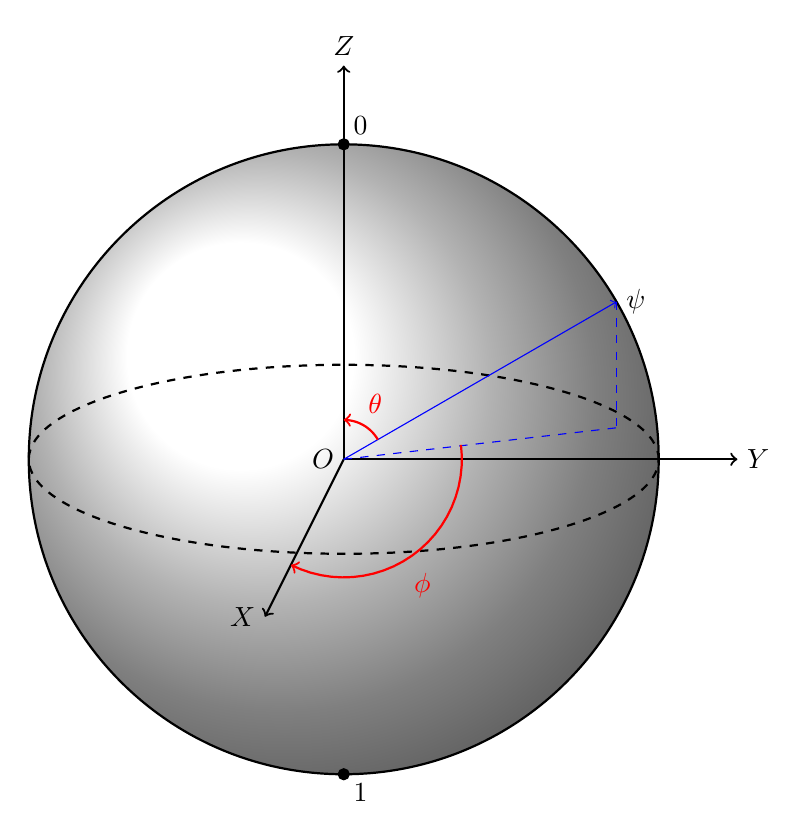
\begin{tikzpicture}
	\def\R{4} % sphere radius
	\fill[ball color=white!50] (0,0) circle (\R); % 3D lighting effect
	\draw[thick] (0,0) circle (4cm);
	\draw[dashed,thick] (0,0) ellipse (4cm and 1.2cm);
	\coordinate (O) at (0,0);
	\coordinate (Z) at (0,5);
	\coordinate (Y) at (5,0);
	\coordinate (X) at (-1,-2);
	\coordinate (V) at (\R*cos{30}, \R*sin{30});
	\coordinate (0) at (0,4);
	\coordinate (1) at (0,-4);
	\coordinate (xc) at (\R*cos{30}, 0.4);
	
	\draw (O) node [left]{$O$};
	\draw (Z) node [above]{$Z$};
	\draw (Y) node [right]{$Y$};
	\draw (X) node [left]{$X$};
	\draw (V) node [right]{$\boldsymbol{\ket{\psi}}$};
	\draw[fill=black] (1) circle (2pt);
	\draw (1) node [below right]{$\boldsymbol{\ket{1}}$};
	\draw[fill=black] (0) circle (2pt);
	\draw (0) node [above right]{$\boldsymbol{\ket{0}}$};
	
	\draw[->,thick] (O) -- (Z);
	\draw[->,thick] (O) -- (Y);
	\draw[->,thick] (O) -- (X);
	
	\draw[dashed, blue] (O) -- (xc);
	\draw[dashed, blue] (V) -- (xc);
	\draw[->, blue] (O) -- (V);
	
	\draw[red] (0.4,0.7) node {$\boldsymbol{\theta}$};
	\draw[red] (1,-1.6) node {$\boldsymbol{\phi}$};
	
	 \draw [->,red,thick,domain=30:90] plot ({0.5*cos(\x)}, {0.5*sin(\x)});
     \draw [->,red,thick,domain=7:-116.5] plot ({1.5*cos(\x)}, {1.5*sin(\x)});
\end{tikzpicture}}
\caption{Vector Representation of Qubit Position}
\label{fig:3Dvector}
\end{figure}
If two vectors are only differing in their global phase, then they are indistinguishable when measuring, i.e. the two vectors below are the same when measured. $$\frac{-1}{\sqrt{2}}\ket{0} + \frac{1}{\sqrt{2}}\ket{1} \equiv \frac{1}{\sqrt{2}}\ket{0} - \frac{1}{\sqrt{2}}\ket{1}$$ When a Hadamard transform is applied, then their relative phases become different and hence the measurements become $\ket{0}$ and $\ket{1}$ respectively. $$\frac{1}{\sqrt{2}}\ket{0} + \frac{1}{\sqrt{2}}\ket{1}, \frac{1}{\sqrt{2}}\ket{0} - \frac{1}{\sqrt{2}}\ket{1}$$  We can now define phase shift gates as the gates which transform an input by rotating it along a certain axis. The base matrices for the rotations in X,Y and Z axis are defined below:
$$X = \begin{pmatrix} 0 & 1 \\ 1 & 0 \end{pmatrix} Y = \begin{pmatrix} 0 & i \\ -i & 0 \end{pmatrix} Z = \begin{pmatrix} 1 & 0 \\ 0 & -1 \end{pmatrix}$$
These are often referred to as Pauli-X Pauli-Y and Pauli-Z gates. More generally, we can have a rotation of a certain angle in the Z axis by using the matrix: $$\begin{pmatrix} 1 & 0 \\ 0 & e^{i\theta} \end{pmatrix},$$ which is commonly referred to the global phase shift gate, denoted as $R_\theta$.
\subsection{Quantum Circuits}
Quantum gates can be applied in a circuit in the same way that classical logic gates can. We use symbols to denote quantum gates as described in Figures \ref{fig:hadamardGate}, \ref{fig:phaseshiftGate}, \ref{fig:measurementGate} and \ref{fig:notGate}, where the lines denote inputs and outputs.
\begin{figure}[!htb]
\centering
\resizebox{2cm}{!}{\Qcircuit @C=1em @R=.7em {
 & \gate{H} & \qw \\
}}
\caption{Quantum circuit describing Hadamard gate}
\label{fig:hadamardGate}
\end{figure}\begin{figure}[!htb]
\centering
\resizebox{2cm}{!}{\Qcircuit @C=1em @R=.7em {
 & \gate{R_\theta} & \qw \\
}}
\caption{Quantum circuit describing phase shift gate by arbitrary angle $\theta$}
\label{fig:phaseshiftGate}
\end{figure}\begin{figure}[!htb]
\centering
\resizebox{2cm}{!}{\Qcircuit @C=1em @R=.7em {
    & \meter & \qw \\
}}
\caption{Quantum circuit describing measurement gate}
\label{fig:measurementGate}
\end{figure}\begin{figure}[!htb]
\centering
\resizebox{2cm}{!}{\Qcircuit @C=1em @R=.7em {
 & \targ & \qw \\
}}
\caption{Quantum circuit describing NOT gate}
\label{fig:notGate}
\end{figure}
\subsubsection{Control Gates and Entanglement}
More commonly in quantum circuits, we use a controlled version of gates. An example of a control gate is the controlled not (CNOT) gate. This gate flips the target qubit if the control qubit is 1, otherwise it leaves it. The controlled not gate is described in Figure \ref{fig:cnotGate}.
\begin{figure}[!htb]
\centering
\resizebox{5cm}{!}{\Qcircuit @C=1em @R=.7em @!R {
\lstick{\ket{0}} & \ctrl{1} & \qw & \ket{0} & & \lstick{\ket{1}} & \ctrl{1} & \qw & \ket{1}\\
\lstick{\ket{0}} & \targ & \qw & \ket{0} & \push{\rule{.3em}{0em}\rule{.3em}{0em}} & \lstick{\ket{0}} & \targ & \qw & \ket{1}
}}
\caption{Quantum circuits describing the effect of controlled not gate on different inputs}
\label{fig:cnotGate}
\end{figure}
The controlled not gate is an example of a multi-input gate, we can mix multi-input gates and single input gates in circuits, and this is required to create \emph{entangled} qubits which are useful in many quantum circuits. Consider the circuit in Figure \ref{fig:entangle}. We have a Hadamard gate acting on a single input, and a controlled not gate which takes the output from the Hadamard transform as its control input.
\begin{figure}[!htb]
\centering
\resizebox{3cm}{!}{\Qcircuit @C=1em @R=.7em {
    \raisebox{-2.5em}{$\ket{I}$} & & \gate{H}  & \ctrl{1} & \qw \\
    & & \qw & \targ & \qw 
}}
\caption{Quantum circuit describing how to create entangled states}
\label{fig:entangle}
\end{figure}
To see exactly what is happening in this circuit, we can split the circuit up, as described in Figure \ref{fig:splitEntangle} 
\begin{figure}[!htb]
\centering
\resizebox{5cm}{!}{\Qcircuit @C=1em @R=.7em {
    \raisebox{-2.5em}{$\ket{I}$} & & \gate{H} & \qw & \raisebox{-2.5em}{$\ket{I'
    }$} & & \ctrl{1} & \qw\\
    & & \qw & \qw & &  & \targ & \qw
}  }
\caption{Quantum circuit for entanglement split into components}
\label{fig:splitEntangle}
\end{figure}
When the circuit is split up in this way, we can describe what transformations are happening at each stage. The first Hadamard transform is only applied to one qubit. Since we have a two qubit input, the second qubit is left unchanged, and the output is only affected by the Hadamard transform on the first qubit. The transformation that a Hadamard gate performs on one qubit is as follows \begin{align*}
    \ket{0} \longrightarrow \frac{1}{\sqrt{2}}(\ket{0} + \ket{1})\\
    \ket{1} \longrightarrow \frac{1}{\sqrt{2}}(\ket{0} - \ket{1})
\end{align*}
When we have a two qubit input, the transformation is as follows:
\begin{align*}
    \ket{00} \longrightarrow \frac{1}{\sqrt{2}}(\ket{00} + \ket{10})\\
    \ket{01} \longrightarrow \frac{1}{\sqrt{2}}(\ket{01} + \ket{11})\\
    \ket{10} \longrightarrow \frac{1}{\sqrt{2}}(\ket{00} - \ket{10})\\
    \ket{11} \longrightarrow \frac{1}{\sqrt{2}}(\ket{01} - \ket{11})
\end{align*}
The matrix for this transformation is:
$$ H_1 = 
\begin{pmatrix}
1 & 0 & 1 & 0\\
0 & 1 & 0 & 1\\
1 & 0 & -1 & 0\\
0 & 1 & 0 & -1
\end{pmatrix}
$$
Since this is the output for the first part of the circuit, the input $\ket{I'}$ it is the input to the next part of the circuit. We can then obtain the matrix for the whole circuit, $M$, by multiplying this first matrix with the matrix for a controlled not gate as follows:
$$
M = N_c\times H_1 = \frac{1}{\sqrt{2}}
\begin{pmatrix}
1 & 0 & 0 & 0\\
0 & 1 & 0 & 0\\
0 & 0 & 0 & 1\\
0 & 0 & 1 & 0
\end{pmatrix}
\begin{pmatrix}
1 & 0 & 1 & 0\\
0 & 1 & 0 & 1\\
1 & 0 & -1 & 0\\
0 & 1 & 0 & -1
\end{pmatrix} = \frac{1}{\sqrt{2}}
\begin{pmatrix}
1 & 0 & 1 & 0\\
0 & 1 & 0 & 1\\
0 & 1 & 0 & -1\\
1 & 0 & -1 & 0
\end{pmatrix}
$$
This matrix is then the transformation for the whole circuit, and transforms states in the following way:
\begin{align*}
    \ket{00} \longrightarrow \frac{1}{\sqrt{2}}(\ket{00} + \ket{11})\\
    \ket{01} \longrightarrow \frac{1}{\sqrt{2}}(\ket{01} + \ket{10})\\
    \ket{10} \longrightarrow \frac{1}{\sqrt{2}}(\ket{00} - \ket{11})\\
    \ket{11} \longrightarrow \frac{1}{\sqrt{2}}(\ket{01} - \ket{10})
\end{align*}
This set of output states is called a \emph{bell state}, and means that if we measure one of the output qubits, we know the value of the other without having to measure it, meaning that the qubits are entangled. Consider the first state: $$\frac{1}{\sqrt{2}}(\ket{00} + \ket{11})$$
If we split this into all possibilities of each qubit with probabilities for each qubit in each state as such:
$$(a\ket{0} + b\ket{1}) \times (c\ket{0} + d\ket{1}),$$
then we can represent all possible output states as
$$ac\ket{00}, ad\ket{01}, bc\ket{10}, bd\ket{11}$$
That means, for our state to be possible, we must have $ad,bc=0$ and $ac,bd=\frac{1}{\sqrt{2}}$, so our qubits are entangled.
\subsubsection{Toffoli Gate}
Typically, classical logic gates such as NAND are irreversible, so they have no quantum representation, however there exists a quantum gate known as the Toffoli gate, invented by Tommaso Toffoli, which can simulate classical logic in a quantum circuit. The toffoli gate takes 3 qubits as input, and outputs 3 qubits. Two of the input qubits are control qubits that are unnaffected by the action of the Toffoli gate, the third qubit is the \emph{target} qubit, which is flipped if both control qubits are in state $\ket{1}$, otherwise it is left alone. The Toffoli gate can be used to simulate NAND gates in quantum circuits, which can then be used in larger circuits to simulate classical arithmetic operations. The truth table, transformation matrix and circuit diagram are shown in Table \ref{table:toffolitruth}, Figure \ref{fig:toffolimatrix} and Figure \ref{fig:toffolicircuit} respectively.
\begin{table}[!htb]
\centering
\begin{tabular}{|c|c|c||c|}
\hline 
\multicolumn{3}{|c||}{Input} & Output \\ 
\hline 
$\ket{a}$ & $\ket{b}$ & $\ket{c}$ & $\ket{c\oplus ab}$ \\ 
\hline 
$\ket{0}$ & $\ket{0}$ & $\ket{0}$ & $\ket{000}$ \\ 
\hline 
$\ket{0}$ & $\ket{0}$ & $\ket{1}$ & $\ket{001}$ \\ 
\hline 
$\ket{0}$ & $\ket{1}$ & $\ket{0}$ & $\ket{010}$ \\ 
\hline 
$\ket{0}$ & $\ket{1}$ & $\ket{1}$ & $\ket{011}$ \\ 
\hline 
$\ket{1}$ & $\ket{0}$ & $\ket{0}$ & $\ket{100}$ \\ 
\hline 
$\ket{1}$ & $\ket{0}$ & $\ket{1}$ & $\ket{101}$ \\ 
\hline 
$\ket{1}$ & $\ket{1}$ & $\ket{0}$ & $\ket{111}$ \\ 
\hline 
$\ket{1}$ & $\ket{1}$ & $\ket{1}$ & $\ket{110}$ \\ 
\hline 
\end{tabular} 
\caption{Truth table for Toffoli transformation}
\label{table:toffolitruth}
\end{table}
\begin{figure}[!htb]
\centering
\resizebox{5cm}{!}{$
\begin{pmatrix}
1 & 0 & 0 & 0 & 0 & 0 & 0 & 0 \\
0 & 1 & 0 & 0 & 0 & 0 & 0 & 0 \\
0 & 0 & 1 & 0 & 0 & 0 & 0 & 0 \\
0 & 0 & 0 & 1 & 0 & 0 & 0 & 0 \\
0 & 0 & 0 & 0 & 1 & 0 & 0 & 0 \\
0 & 0 & 0 & 0 & 0 & 1 & 0 & 0 \\
0 & 0 & 0 & 0 & 0 & 0 & 0 & 1 \\
0 & 0 & 0 & 0 & 0 & 0 & 1 & 0 
\end{pmatrix}
$}
\caption{Matrix representing Toffoli transformation}
\label{fig:toffolimatrix}
\end{figure}
\begin{figure}[!htb]
\centering
\resizebox{1.5cm}{!}{\Qcircuit @C=1em @R=.7em @!R {
\lstick{\ket{a}} & \ctrl{1} & \rstick{\ket{a}} \qw \\
\lstick{\ket{a}} & \ctrl{1} & \rstick{\ket{b}} \qw \\
\lstick{\ket{a}} & \targ & \rstick{\ket{c\oplus ab}} \qw
}}
\caption{Circuit representing Toffoli transformation}
\label{fig:toffolicircuit}
\end{figure}
\subsection{Quantum Fourier Transform}
Another key example of a quantum logic circuit which is used in many quantum algorithms is the Quantum Fourier transform (QFT). This is a quantum version of the classical Fast Fourier transform (FFT), and can be recreated in a quantum circuit with a collection of gates. The QFT allows us to find the underlying periodic behaviour of a function, and so it is useful in many quantum algorithms.
\subsubsection{Discrete Fourier Transform} 
To understand how the Quantum Fourier transform allows us to find the period of a function, we can look at the classical discrete Fourier transform. The discrete Fourier transform essentially allows us to take a finite sequence of equally spaced samples of an input function with high noise (irregularities from the base function) and find the underlying periodic behaviour. This transformation is useful because it can break down a seemingly random signal composed of many different frequency waves into its component parts. The transformation is done using properties of sinusoidal waves and Euler's formula.
For a simple example of the discrete Fourier transform, we can apply it to a sample of a sine wave with frequency 1Hz and amplitude 1:
\begin{figure}[!htb]
\centering
\resizebox{7cm}{!}{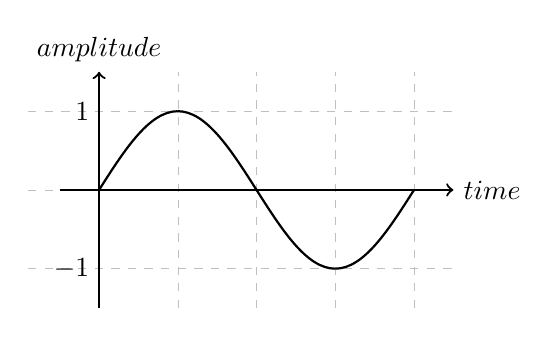
\begin{tikzpicture}
\draw[help lines, color=gray!50, dashed ] (-0.9,-1.5) grid (4.5,1.5);
\draw[->,thick] (-0.5,0)--(4.5,0) node[right]{$time$};
\draw[->,thick] (0,-1.5)--(0,1.5) node[above]{$amplitude$};
\draw(0,1) node[left] {$1$};
\draw(0,-1) node[left] {$-1$};
\draw[thick] (0,0) sin (1,1);
\draw[thick] (1,1) cos (2,0);
\draw[thick] (2,0) sin (3,-1);
\draw[thick] (3,-1) cos (4,0);
\end{tikzpicture}}
\caption{Sine wave with frequency 1Hz and amplitude 1}
\label{fig:sine}
\end{figure}
We can take samples of this function's amplitude at equally spaced points. For this example we use a sampling frequency of 8 Hz:
\begin{figure}[!htb]
\centering
\resizebox{7cm}{!}{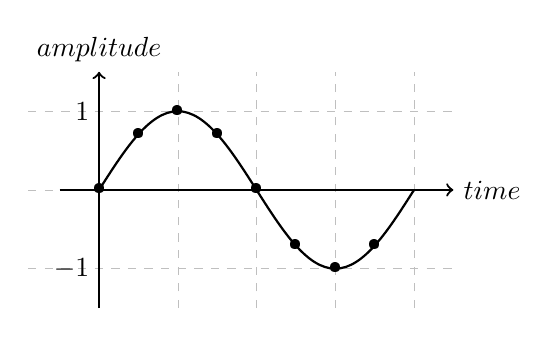
\begin{tikzpicture}
\draw[help lines, color=gray!50, dashed ] (-0.9,-1.5) grid (4.5,1.5);
\draw[->,thick] (-0.5,0)--(4.5,0) node[right]{$time$};
\draw[->,thick] (0,-1.5)--(0,1.5) node[above]{$amplitude$};
\draw(0,1) node[left] {$1$};
\draw(0,-1) node[left] {$-1$};
\draw[thick] (0,0) sin (1,1);
\draw[thick] (1,1) cos (2,0);
\draw[thick] (2,0) sin (3,-1);
\draw[thick] (3,-1) cos (4,0);
\foreach \Point in {(0,0),(0.5,0.707),(1,1),(1.5,0.707),(2,0),(2.5,-0.707),(3,-1),(3.5,-0.707)}{
    \node at \Point {\textbullet};
}
\end{tikzpicture}}
\caption{Sine wave sampled at 8Hz}
\label{fig:sineSample}
\end{figure}
The eight values for amplitude we get are displayed in Table \ref{table:amplitudes}
\begin{table}[!htb]
\centering
\begin{tabular}{ |c|c| } 
\hline
 & amplitude \\
\hline
$x_0$ & 0 \\ 
$x_1$ & 0.707 \\ 
$x_2$ & 1 \\ 
$x_3$ & 0.707 \\ 
$x_4$ & 0 \\ 
$x_5$ & -0.707 \\ 
$x_6$ & -1 \\ 
$x_7$ & -0.707 \\ 
\hline
\end{tabular}
\caption{Amplitudes of samples}
\label{table:amplitudes}
\end{table}
Using these values and the formula for the discrete Fourier transform, we can work out the frequency bins for each value by substituting in the values for k, n and $x_i$. When this is done, we get values for $X_k$ as shown in Table \ref{table:fourierCoefficient}
\begin{table}[!htb]
\centering
\begin{tabular}{ |c|c| } 
\hline
& Fourier Coefficient \\
\hline
$X_0$ & 0 \\ 
$X_1$ & 0 - 4\textit{i} \\ 
$X_2$ & 0 \\ 
$X_3$ & 0 \\ 
$X_4$ & 0 \\ 
$X_5$ & 0 \\ 
$X_6$ & 0 \\ 
$X_7$ & 0 + 4\textit{i} \\ 
\hline
\end{tabular}
\caption{Fourier Coefficients of samples}
\label{table:fourierCoefficient}
\end{table}
From this we can see that the only non-zero values are those for $X_1$ and $X_7$. We choose to take the magnitude of these rather than the full complex number for reasons that will be shown later. We can plot this as a frequency against magnitude graph as shown in Figure \ref{fig:nyquist}
\begin{figure}[!htb]
\centering
\resizebox{10cm}{!}{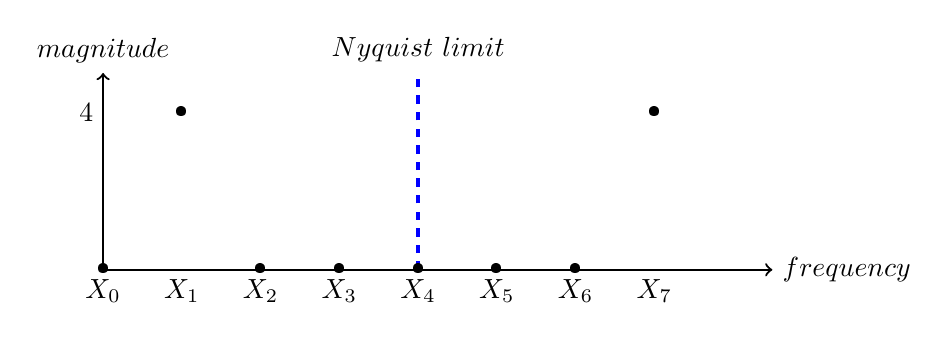
\begin{tikzpicture}
\draw[->,thick] (0,0)--(8.5,0) node[right]{$frequency$};
\draw[->,thick] (0,0)--(0,2.5) node[above]{$magnitude$};
\draw(0,2) node[left] {$4$};
\draw(0,0) node[below] {$X_0$};
\draw(1,0) node[below] {$X_1$};
\draw(2,0) node[below] {$X_2$};
\draw(3,0) node[below] {$X_3$};
\draw(4,0) node[below] {$X_4$};
\draw(5,0) node[below] {$X_5$};
\draw(6,0) node[below] {$X_6$};
\draw(7,0) node[below] {$X_7$};
\draw[ultra thick, blue, dashed] (4,0)--(4,2.5) node[black, above]{$Nyquist$ $limit$};
\foreach \Point in {(0,0),(1,2),(2,0),(3,0),(4,0),(5,0),(6,0),(7,2)}{
    \node at \Point {\textbullet};
}
\end{tikzpicture}}
\caption{Frequency against magnitude plot for sample}
\label{fig:nyquist}
\end{figure}
The Nyquist limit is the highest frequency that can be coded at a given sampling rate to be able to fully reconstruct the original signal, and it is equal to $\frac{N}{2}$~\cite{tretter1976introduction}. Due to this, we remove all values above the Nyquist limit, and double all values below the Nyquist limit to account for the removed values. This leaves us with a result for only $X_1$, being a magnitude of 2*4 = 8. To get the amplitude of the original sample, we divide this amplitude by the number of samples. In this case we have $\frac{8}{8}$ which tells us that the amplitude of the original sample was 1. To find the frequency of the original sample, we have to look at the value of k. In this case it is 1, so our frequency was 1 Hz. We can also calculate the phase that this sinusoidal wave was shifted compared to a normal cosine wave. In order to do this we need to look at the complex number we obtained for $X_k$, which in this case was $0-8\textit{i}$. If we plot this on a complex plane we get an angle from the positive real axis to the plot, as shown in Figure \ref{fig:complex}
\begin{figure}[!htb]
\centering
\resizebox{6cm}{!}{\begin{tikzpicture}
\draw[->,thick] (-2.5,0)--(2.5,0) node[right]{$real$};
\draw[->,thick] (0,-2.5)--(0,2.5) node[above]{$imaginary (i)$};
\draw[->,ultra thick, orange] (0,0)--(0,-2) node[left, black]{$0-8i$};
\coordinate (x) at (1.5,0);
\coordinate (y) at (0,0);
\coordinate (z) at (270:1);
\pic[draw,pic text=$\theta$,angle radius=20pt,angle eccentricity=1.3,->, thick]{angle=x--y--z};
\end{tikzpicture}}
\caption{Angle between positive real axis and sample}
\label{fig:complex}
\end{figure}
The angle $\theta$ is equal to $\frac{3\pi}{2}$, which is our phase shift from a normal cosine wave. This method can be used for any type of sample, and the results will be normalised against a cosine wave, so we can use it for statistical analysis of the sample.
\begin{figure}[!htb]
\centering
\resizebox{8cm}{!}{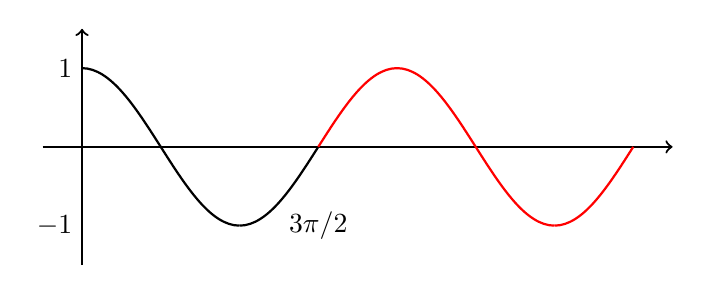
\begin{tikzpicture}
\draw[->,thick] (-0.5,0)--(7.5,0);
\draw[->,thick] (0,-1.5)--(0,1.5);
\draw(0,1) node[left] {$1$};
\draw(0,-1) node[left] {$-1$};
\draw[thick] (0,1) cos (1,0);
\draw[thick] (1,0) sin (2,-1);
\draw[thick] (2,-1) cos (3,0);
\draw[thick, red] (3,0) sin (4,1);
\draw[thick, red] (4,1) cos (5,0);
\draw[thick, red] (5,0) sin (6,-1);
\draw[thick, red] (6,-1) cos (7,0);
\draw(3,-1) node[] {$3\pi/2$};
\end{tikzpicture}}
\caption{Phase shift of sample from cosine wave}
\label{fig:phase}
\end{figure}
\subsubsection{Applying the Quantum Fourier Transform}
The Quantum Fourier transform (QFT) works in a similar way as the discrete fourier transform, with the one major difference being that the QFT takes quantum states as inputs and outputs. It takes the quantum state $\ket{x} = \sum_{j=0}^{N-1}x_j\ket{i}$ and maps it to the quantum state  $\sum_{k=0}^{N-1}y_k\ket{k}$ according to the formula:
$$y_k = \frac{1}{\sqrt{N}}\sum_{j=0}^{N-1}x_j\cdot{e^{2\pi ijk/N}}$$
Consider the 2-qubit state $\ket{x} = a_0\ket{00} + a_1\ket{01} + a_2\ket{10} + a_3\ket{11}$, in this state, then we have $N = 2^2 = 4$. We can apply the QFT to each instance by subsituting in k as 0,1,2,3 respectively as follows:
$$y_0 = \frac{1}{2}\sum_{j=0}^{3}a_j=\frac{1}{2}(a_{00}+a_{01}+a_{10}+a_{11})$$
$$y_1 = \frac{1}{2}\sum_{j=0}^{3}a_j\cdot{\omega^j}=\frac{1}{2}(a_{00}+a_{01}\cdot{\omega}+a_{10}\cdot{\omega^2}+a_{11}\cdot{\omega^3})$$
$$y_2 = \frac{1}{2}\sum_{j=0}^{3}a_j\cdot{\omega^2j}=\frac{1}{2}(a_{00}+a_{01}\cdot{\omega^2}+a_{10}\cdot{\omega^4}+a_{11}\cdot{\omega^6})$$
$$y_3 = \frac{1}{2}\sum_{j=0}^{3}a_j\cdot{\omega^3j}=\frac{1}{2}(a_{00}+a_{01}\cdot{\omega^3}+a_{10}\cdot{\omega^6}+a_{11}\cdot{\omega^9})$$
These values can be represented in a matrix form as shown below:
$$F = \frac{1}{2}
\begin{pmatrix} 
1 & 1 & 1 & 1 \\
1 & \omega & \omega^2 & \omega^3 \\
1 & \omega^2 & \omega^4 & \omega^6 \\
1 & \omega^3 & \omega^6 & \omega^9 \\
\end{pmatrix} = \frac{1}{2} 
\begin{pmatrix}
1 & 1 & 1 & 1 \\
1 & \omega & \omega^2 & \omega^3 \\
1 & \omega^2 & 1 & \omega^2 \\
1 & \omega^3 & \omega^2 & \omega \\
\end{pmatrix} = \frac{1}{2} 
\begin{pmatrix}
1 & 1 & 1 & 1 \\
1 & i & -1 & -i \\
1 & -1 & 1 & -1 \\
1 & -i & -1 & i \\
\end{pmatrix}
$$
\subsubsection{Quantum Fourier Transform Circuit}
The Quantum Fourier transform can be represented as a quantum circuit, and we can prove that this performs the same transformation that we just obtained by observing the matrix for the transformation of the whole circuit. The QFT for a two qubit circuit is shown in Figure \ref{fig:qft2qubit}.
\begin{figure}[!htb]
\centering
\resizebox{5cm}{!}{\Qcircuit @C=1em @R=.7em {
    & \gate{H} & \gate{R_2} & \qw & \qswap & \qw \\
    & \qw & \ctrl{-1} & \gate{H} & \qswap \qwx & \qw
}}
\caption{Quantum Fourier Transform for a 2-qubit circuit}
\label{fig:qft2qubit}
\end{figure}
The gate at the end is called a \emph{swap} gate, and simply swaps the order of the qubits. This transformation is then as follows:
\begin{align*}
    \ket{00} \longrightarrow \ket{00}\\
    \ket{01} \longrightarrow \ket{10}\\
    \ket{10} \longrightarrow \ket{01}\\
    \ket{11} \longrightarrow \ket{11}
\end{align*}
and can be represented in matrix form as:
$$
\begin{pmatrix}
1 & 0 & 0 & 0\\
0 & 0 & 1 & 0\\
0 & 1 & 0 & 0\\
0 & 0 & 0 & 1
\end{pmatrix}
$$
Other than the swap gate, we have a Hadamard transform acting on the first qubit only, then a controlled phase shift of order 2, then another Hadamard transform acting on the second qubit only. The generalised matrix for the controlled phase shift gate can be represented as:
$$
R_k = 
\begin{pmatrix}
1 & 0 & 0 & 0\\
0 & 1 & 0 & 0\\
0 & 0 & 0 & 1\\
0 & 0 & 0 &e^{2\pi i/2k}
\end{pmatrix}
$$
Therefore, the matrix for the $R_2$ gate is:
$$
R_2 = 
\begin{pmatrix}
1 & 0 & 0 & 0\\
0 & 1 & 0 & 0\\
0 & 0 & 0 & 1\\
0 & 0 & 0 & i
\end{pmatrix}
$$
We can then split the circuit into its seperate components as shown in Figure \ref{fig:qft2qubitsplit}, and represent it as a series of matrix multiplications which take the input from $\ket{I}$ to $\ket{A}$, $\ket{B}$, $\ket{C}$, and finally $\ket{O}$ respectively. 
\begin{figure}[!htb]
\centering
\resizebox{8cm}{!}{\Qcircuit @C=1em @R=.7em {
    \raisebox{-2.5em}{$\ket{I}$} & & \gate{H} & \qw  & \raisebox{-2.5em}{$\ket{A}$} & &\gate{R_2} & \qw & \raisebox{-2.5em}{$\ket{B}$} & & \qw & \qw & \raisebox{-2.5em}{$\ket{C}$} & & \qswap & \qw & \raisebox{-2.5em}{$\ket{O}$} \\
    & & \qw & \qw &  & & \ctrl{-1} & \qw &  & & \gate{H} & \qw & & &  \qswap \qwx & \qw &
}}
\caption{Quantum Fourier Transform for a 2-qubit circuit split into components}
\label{fig:qft2qubitsplit}
\end{figure}
These matrices can be denoted as $H_1$, $R_c(2)$, $H_2$, and $swap$ respectively. When we multiply these matrices out:
\begin{align*}
M &= swap \times H_2 \times R_c(2) \times H_1\\
&=
\begin{pmatrix}
1 & 0 & 0 & 0\\
0 & 0 & 1 & 0\\
0 & 1 & 0 & 0\\
0 & 0 & 0 & 1
\end{pmatrix} 
\frac{1}{\sqrt{2}}
\begin{pmatrix}
1 & 1 & 0 & 0\\
1 & -1 & 0 & 0\\
0 & 0 & 1 & 1\\
0 & 0 & 1 & -1
\end{pmatrix}
\begin{pmatrix}
1 & 0 & 0 & 0\\
0 & 1 & 0 & 0\\
0 & 0 & 1 & 0\\
0 & 0 & 0 & i
\end{pmatrix}
\frac{1}{\sqrt{2}}
\begin{pmatrix}
1 & 0 & 1 & 0\\
0 & 1 & 0 & 1\\
1 & 0 & -1 & 0\\
0 & 1 & 0 & -1
\end{pmatrix},
\end{align*}
we can obtain the matrix for the whole circuit as:
$$
\frac{1}{2}
\begin{pmatrix}
1 & 1 & 1 & 1\\
1 & i & -1 & -i\\
1 & -1 & 1 & - 1\\
1 & -i & -1 & i
\end{pmatrix}
$$
We can see that indeed this is the same matrix as the one we obtained earlier, proving that this circuit performs the QFT for a two qubit circuit.
This circuit can be extended to a circuit with any number of input and output qubits as described in Figure \ref{fig:QFTnQubit}, and we can denote it in a larger circuit as a single gate to make things simpler using the notation in Figure \ref{fig:QFTgate}.
\begin{figure}[!htb]
\centering
\resizebox{\linewidth}{!}{\Qcircuit @C=1em @R=.7em @!R {
    \lstick{\ket{I_1}} & \gate{H} & \gate{R_2} & \qw & \cdots & &  \gate{R_{n-1}} & \gate{R_n} & \qw & \qw & \qw & \qw & \qw & \qw & \qw & \qw & \qw & \qw & \qw & \qw & \qw & \qswap & \qw & \qw & \qw & \qw & \raisebox{-10em}{$\ket{O}$}\\
    \lstick{\ket{I_2}} & \gate{H} & \ctrl{-1} & \qw & \cdots & & \qw & \qw & \qw & \gate{H} & \qw &  \cdots & & \gate{R_{n-2}} & \gate{R_{n-1}} & \qw & \cdots & & \qw & \qw & \qw & \qw \qwx & \qswap & \qw & \qw & \qw \\
    \lstick{\vdotswithin{I_{n-1}}} & & \vdotswithin{} & & & & & & & & & & & & & & & & & & & \qwx & \qwx & & \vdotswithin{} \\
    \lstick{\ket{I_{n-1}}} & \qw & \qw & \qw & \qw & \qw & \ctrl{-3} & \qw & \qw & \qw & \qw & \qw & \qw & \ctrl{-2} & \qw & \qw & \cdots & & \gate{H} & \gate{R_2} & \qw & \qw \qwx & \qswap \qwx & \qw & \qw & \qw \\
    \lstick{\ket{I_n}} & \qw & \qw & \qw & \qw & \qw & \qw & \ctrl{-4} & \qw & \qw & \qw & \qw & \qw & \qw & \ctrl{-3} & \qw & \cdots & & \qw & \ctrl{-1} & \gate{H} & \qswap \qwx & \qw & \qw & \qw & \qw
}}
\caption{Quantum Fourier Transform for a n-qubit circuit}
\label{fig:QFTnQubit}
\end{figure}
\begin{figure}[!htb]
\centering
\resizebox{3cm}{!}{\Qcircuit @C=1em @R=.7em @!R {
\raisebox{-5em}{$\ket{I}$} & & \multigate{3}{QFT} & \qw & \raisebox{-5em}{$\ket{O}$}\\
& & \ghost{QFT} & \qw & \\
& & \ghost{QFT} & \qw & \\
& & \ghost{QFT} & \qw & 
}}
\caption{Quantum Fourier Transform gate}
\label{fig:QFTgate}
\end{figure}
\subsection{Shor's Algorithms}
In his paper: \emph{Polynomial-Time Algorithms for Prime Factorization and Discrete Logarithms on a Quantum Computer}~\cite{shor1999polynomial}, Peter W. Shor introduced two algorithms which are able to solve the prime factorisation problem and the discrete logarithm problem respectively in polynomial time. The algorithms both involve reducing the problem of finding either a prime factor or a discrete logarithm into a period finding problem, which can be completed on a quantum computer. The algorithms involve a number of steps which can be computed on a classical computer to avoid unnecessary complexity in the quantum circuit. The hardest part of the computation is calculating the period of the function which the problem can be reduced to.
\subsubsection{Shor's Algorithm for Prime Factorisation}
Shor's Algorithm for prime factorisation can be summarised in 5 steps. Suppose we have a number $N$, which has the factors $p$ and $q$: \\
1. If $N$ is even, prime or a prime power, there exists classical algorithms to calculate factorisation so exit.\\
2. Choose a random number $a$ < $N$ and calculate $\gcd(a,N)$, if this is not equal to 1, then we have found a factor of $N$ in $a$, so exit.\\
3. Find the period $r$ of the function$f(x) = a^x\mod N$. (This is the quantum aspect of the algorithm)\\
4. If $r$ is odd, or $a^{r/2}\mod N = -1\mod N$ then go back to step 1.\\
5. $\gcd(a^{r/2}\pm 1, N)$ are prime factors of $N$\\
Since we already have fast algorithms to calculate the classical parts of Shor's algorithm, this section will describe how we can use the properties of quantum computation to calculate the period of the function $f(x) = a^x\mod N$.
\subsubsection{Phase Estimation}
For some unitary operation on quantum state: $U\ket{\psi}$, if it is known that the state $\ket{\psi}$ is an \emph{eigenstate} of that operator, i.e. the quantum state does not change when it is operated on by $U$, then there exists a corresponding complex eigenvalue such that $U\ket{\psi} \equiv e^{2\pi i\phi}\ket{\psi}$, $0 \leq \phi < 1$~\cite{nielsen2002quantum}. We can design quantum circuits to estimate this value of $\phi$ to a certain number of decimal places. If we know both the value of $U$ and $\ket{\psi}$, we can estimate $\phi$ using the circuit described in Figure \ref{fig:phaseEstimationCircuit}.
\begin{figure}[!htb]
\centering
\hspace{-2.5cm}
\resizebox{10cm}{!}{\Qcircuit @C=1em @R=.7em @!R {
    & & \lstick{\ket{0}} & \gate{H} & \qw & \qw & \qw & \cdots & & \qw & \ctrl{6} & \rstick{\frac{1}{\sqrt{2}}(\ket{0} + e^{2\pi i(2^{m-1}\phi)}\ket{1}}) \qw \\
    & & \lstick{\ket{0}} & \gate{H} & \qw & \qw & \qw & \cdots & & \ctrl{5} & \qw & \rstick{\frac{1}{\sqrt{2}}(\ket{0} + e^{2\pi i(2^{m-2}\phi)}\ket{1}}) \qw \\
    & & \lstick{\vdotswithin{\ket{0}}} & \vdotswithin{} & & & & & & \\
    & & \lstick{\ket{0}} & \gate{H} & \qw & \ctrl{3} & \qw & \cdots & & \qw & \qw & \rstick{\frac{1}{\sqrt{2}}(\ket{0} + e^{2\pi i(2^{1}\phi)}\ket{1}}) \qw \\
    & & \lstick{\ket{0}} & \gate{H} & \ctrl{2} & \qw & \qw & \cdots & & \qw & \qw & \rstick{\frac{1}{\sqrt{2}}(\ket{0} + e^{2\pi i(2^{0}\phi)}\ket{1}}) \qw \\
    & & & & & \\
    & & \lstick{\raisebox{-6.8em}{$\ket{\psi}$}} & \qw & \multigate{3}{U^{2^0}} & \multigate{3}{U^{2^1}} & \qw & \cdots & & \multigate{3}{U^{2^{m-1}}} & \multigate{3}{U^{2^{m-1}}} & \rstick{\raisebox{-6.8em}{$\ket{\psi}$}} \qw \\
    & &  & \qw & \ghost{U^{2^0}} & \ghost{U^{2^1}} & \qw & \cdots & & \ghost{U^{2^{m-2}}} & \ghost{U^{2^{m-1}}} & \qw \\
    & &  & \qw & \ghost{U^{2^0}} & \ghost{U^{2^1}} & \qw & \cdots & & \ghost{U^{2^{m-2}}} & \ghost{U^{2^{m-1}}} & \qw \\
    & & & \qw & \ghost{U^{2^0}} & \ghost{U^{2^1}} & \qw & \cdots & & \ghost{U^{2^{m-2}}} & \ghost{U^{2^{m-1}}} & \qw \\
    {\inputgroupv{1}{5}{1em}{4em}{R_1}} \\ {\inputgroupv{7}{10}{1em}{3.1em}{R_2}} \\
}}
\caption{Phase Estimation Circuit~\cite{cleve1998quantum}}
\label{fig:phaseEstimationCircuit}
\end{figure}
This circuit involves two registers of qubits, $R_1$ and $R_2$. Register 1 contains $n$ qubits which are put into a superposition of all states using a series of parallel Hadamard transforms, i.e. the first register is initially in the state: $$\frac{1}{\sqrt{2^n}}\sum_{y=0}^{2^m-1}\ket{y}$$
Register 2 contains $m$ controlled U gates, each of which performs the square of the operation before it. The result of this is that the first register is put into a superposition of all values of our function. The state of the first register becomes: 
$$\frac{1}{\sqrt{2}}((\ket{0} + e^{2\pi i (2^{0} \phi} \ket{1})(\ket{0} + e^{2\pi i (2^{1} \phi} \ket{1})(\ket{0} + e^{2\pi i (2^{m-2} \phi} \ket{1})(\ket{0} + e^{2\pi i (2^{m-1} \phi} \ket{1}))$$
$$=\frac{1}{\sqrt{2^m}}\sum_{y=0}^{2^m-1}e^{2\pi i \phi y}\ket{y}$$
recall that the Quantum Fourier transform can be represented as 
$$\sum_{j=0}^{N-1}x_j\ket{i} \longrightarrow \sum_{k=0}^{N-1}y_k\ket{k},$$
where 
$$y_k = \frac{1}{\sqrt{N}}\sum_{j=0}^{N-1}x_j\cdot{e^{2\pi ijk/N}}$$
This means that, because $N = 2^m$ in our example, if we apply the \emph{inverse} of the QFT to this output, we get the state $\ket{2^m\phi}$ in our first register of $n$ qubits, and so we can measure the phase. The numbers of qubits needed in registers 1 and 2 are $n = 2\log_2 N$ and $m = \log_2 N$ respectively~\cite{kendon2004entanglement}.
\subsubsection{Quantum Circuit for Prime Factorisation}
The problem for finding the period of a function can be reformulated into a phase estimation problem. If we want to find the period $r$ of a function $$f(x) = a^x\mod N,$$ and we have a unitary operator which performs: $$U\ket{y} \longrightarrow \ket{xy\mod N},$$ which, as discussed in the previous section, can be replaced by its eigenvalue and eigenvector as such: $$e^{2\pi i\phi}\ket{\psi_s}$$ In fact, there are $r$ eigenvectors with corresponding eigenvalues, so $\ket{\psi_s}$ just denotes one of these eigenvectors. These eigenvalues can be represented as $e^{2\pi is/r}$~\cite{nielsen2002quantum}, which means that if we can measure the phase using our phase estimation circuit, we have a value for $\frac{s}{r}$. We do not need to know the specific eigenvector $\ket{\psi_s}$, as we can just put the system in a superposition of all possible vectors, and thus containing all $r$ eigenvectors. If we run a simulation representing this circuit, we see that the probability distribution forms peaks, these peaks correspond to each eigenvector, so it is more likely that when we take a measurement, we will measure the value of one of these peaks, which will give us a correct value for $r$. An example of the full circuit needed to factor 21 is described in Figure \ref{fig:shors21}. The next section will describe a practical example of how we can obtain the factors of a number using Shor's algorithm.
\begin{figure}[!htb]
\centering
\resizebox{10cm}{!}{\Qcircuit @C=1em @R=.7em @!R {
    & & \lstick{\ket{0}} & \gate{H} & \qw & \qw & \qw & \qw & \qw & \qw & \qw & \qw & \qw & \ctrl{11} & \multigate{9}{QFT^\dag} & \meter \\
    & & \lstick{\ket{0}} & \gate{H} & \qw & \qw & \qw & \qw & \qw & \qw & \qw & \qw & \ctrl{10} & \qw & \ghost{QFT^\dag} & \meter \\
    & & \lstick{\ket{0}} & \gate{H} & \qw & \qw & \qw & \qw & \qw & \qw & \qw & \ctrl{9} & \qw & \qw & \ghost{QFT^\dag} & \meter \\
    & & \lstick{\ket{0}} & \gate{H} & \qw & \qw & \qw & \qw & \qw & \qw & \ctrl{8} & \qw & \qw & \qw & \ghost{QFT^\dag} & \meter \\
    & & \lstick{\ket{0}} & \gate{H} & \qw & \qw & \qw & \qw & \qw & \ctrl{7} & \qw & \qw & \qw & \qw & \ghost{QFT^\dag} & \meter \\
    & & \lstick{\ket{0}} & \gate{H} & \qw & \qw & \qw & \qw & \ctrl{6} & \qw & \qw & \qw & \qw & \qw & \ghost{QFT^\dag} & \meter \\
    & & \lstick{\ket{0}} & \gate{H} & \qw & \qw & \qw & \ctrl{5} & \qw & \qw & \qw & \qw & \qw & \qw & \ghost{QFT^\dag} & \meter \\
    & & \lstick{\ket{0}} & \gate{H} & \qw & \qw & \ctrl{4} & \qw & \qw & \qw & \qw & \qw & \qw & \qw & \ghost{QFT^\dag} & \meter \\
    & & \lstick{\ket{0}} & \gate{H} & \qw & \ctrl{3} & \qw & \qw & \qw & \qw & \qw & \qw & \qw & \qw & \ghost{QFT^\dag} & \meter \\
    & & \lstick{\ket{0}} & \gate{H} & \ctrl{2} & \qw & \qw & \qw & \qw & \qw & \qw & \qw & \qw & \qw & \ghost{QFT^\dag} & \meter \\
    & & & & & \\
    & & \lstick{\ket{1}} & \qw & \multigate{4}{U^{2^0}} & \multigate{4}{U^{2^1}} & \multigate{4}{U^{2^2}} & \multigate{4}{U^{2^3}} & \multigate{4}{U^{2^4}} & \multigate{4}{U^{2^5}} & \multigate{4}{U^{2^6}} & \multigate{4}{U^{2^7}} & \multigate{4}{U^{2^8}} & \multigate{4}{U^{2^9}}  & \qw & \rstick{\ket{1}} \qw \\
    & & \lstick{\ket{1}} & \qw & \ghost{U^{2^0}} & \ghost{U^{2^1}} & \ghost{U^{2^2}} & \ghost{U^{2^3}} & \ghost{U^{2^4}} & \ghost{U^{2^5}} & \ghost{U^{2^6}} & \ghost{U^{2^7}} & \ghost{U^{2^8}} & \ghost{U^{2^9}} & \qw & \rstick{\ket{1}} \qw \\
    & & \lstick{\ket{1}} & \qw & \ghost{U^{2^0}} & \ghost{U^{2^1}}& \ghost{U^{2^2}} & \ghost{U^{2^3}} & \ghost{U^{2^4}} & \ghost{U^{2^5}} & \ghost{U^{2^6}} & \ghost{U^{2^7}}& \ghost{U^{2^8}} & \ghost{U^{2^9}} & \qw & \rstick{\ket{1}} \qw \\
    & & \lstick{\ket{1}} & \qw & \ghost{U^{2^0}} & \ghost{U^{2^1}} & \ghost{U^{2^2}} & \ghost{U^{2^3}} & \ghost{U^{2^4}} & \ghost{U^{2^5}} & \ghost{U^{2^6}} & \ghost{U^{2^7}}& \ghost{U^{2^8}} & \ghost{U^{2^9}} & \qw & \rstick{\ket{1}} \qw \\
    & & \lstick{\ket{1}} & \qw & \ghost{U^{2^0}} & \ghost{U^{2^1}} & \ghost{U^{2^2}} & \ghost{U^{2^3}} & \ghost{U^{2^4}} & \ghost{U^{2^5}} & \ghost{U^{2^6}} & \ghost{U^{2^7}}& \ghost{U^{2^8}} & \ghost{U^{2^9}} & \qw & \rstick{\ket{1}} \qw \\
    {\inputgroupv{1}{10}{1em}{9em}{R_1}} \\ {\inputgroupv{12}{16}{1em}{4em}{R_2}} \\
}}
\caption{Quantum Circuit to Factorise 21}
\label{fig:shors21}
\end{figure}
\subsubsection{Example of Factorisation Using Shor's Algorithm}
Using the software {LIQU}i|>~\cite{1402.4467}, we were able to simulate a quantum circuit which would implement Shor's factorisation algorithm. When our input $N$ was 253, and a value of $a$ as 2, we obtained a measurement of $\ket{0001000001001010} = 4170$. Using the continued fraction algorithm described in Box 5.3 from \cite{nielsen2002quantum}, we can represent $\frac{4170}{2^{16}} = \frac{4170}{65536}$ as: $$0 + \frac{1}{15 + \frac{1}{1 + \frac{1}{2 + \frac{1}{1 + \frac{1}{1 + \frac{1}{10 + \frac{1}{1 + \frac{1}{7 + \frac{1}{1 + \frac{1}{2}}}}}}}}}}$$ with values for $d$ and $r$ as described in Table \ref{table:valuesdr}.
\begin{table}[!htb]
\centering
\begin{tabular}{|c|c|c|c|c|c|c|c|c|c|c|}
\hline
$d$ & 1  & 1  & 3  & 4  & 7   & 74   & 81   & 641   & 722   & 2085  \\ \hline
$r$ & 15 & 16 & 47 & 63 & 110 & 1163 & 1273 & 10074 & 11347 & 32768 \\ \hline
\end{tabular}
\caption{Values for $d$ and $r$ obtained from continued fraction algorithm [Box 5.3]~\cite{nielsen2002quantum}}
\label{table:valuesdr}
\end{table}
Equation 5.3 in Shor's paper describes how we can obtain the value for $r$ from this set of values. There is at most one fraction $d/r$ with $r < N$ which satisfies the equation: $$\abs*{\frac{c}{q} - \frac{d}{r}} < \frac{1}{2q},$$ where $q$ is the power of 2 with $n^2 \leq q < 2n^2$, equal to $2^{16} = 65536$, and c is our observed value = 4170. Therefore the only values which satisfy this requirement in the table are $d = 7$ and $r = 110$. So we have obtained a value for the period of the function, $r$, as 110, now we can perform the last two steps in Shor's algorithm to calculate the factors of 253. Since $r$ is even and $a^{r/2}\mod N = 2^{55}\mod 253 = 208 \neq -1\mod 253$, our value for $r$ is correct. We can then obtain factors for 253 as $gcd(2^{55}\pm 1\mod 253, 253)$ which are 11 and 23 respectively. We can verify that $11\times 23$ is indeed equal to 253, so we have correctly obtained the prime factors of 253.
\subsubsection{Shor's Algorithm for Discrete Logarithms}
Shor's paper also describes an algorithm for solving the discrete logarithm problem for prime groups. This algorithm can be extended to solve the discrete logarithm problem for a generic cyclic group $G$ which has some generator $g$, and a group operation $\odot$, given that the group operation can be applied multiple times efficiently using quantum circuits~\cite{ekeraa2016modifying}. For a generic group such as this, we denote the process of applying the group operation a number $d$ of times to an initial element as $x = d[g]$, thus the discrete logarithm problem for a generic group such as this, is to find the discrete logarithm $d$ given $g$ and $x$. The algorithm below describes how we can solve this problem using a quantum subroutine, taken from \cite{ekeraa2016modifying}.\\
1. Use a quantum circuit to calculate a "good pair", $(j,k)$, on input of a generator $g$ and an element $x$ of the group $G$. This good pair is what we can use in the next step to calculate the discrete logarithm from\\
2. Using a classical algorithm, compute $d$ from this good pair $(j,k)$ using the equivalence:
$$d \equiv \round{\frac{kq}{2^l}}t^{-1}\mod q,$$ where $l$ is the length of the qubit registers in the quantum circuit, $q$ is the order of the group and $t$ is an integer that satisfies:
$$t = \frac{\{jq\}_{2^l}-jq}{2^l}\in \mathbb{Z}$$
\subsubsection{Quantum Subroutine to Compute a Good Pair}
This section will outline the quantum algorithm described in \cite{ekeraa2016modifying}, that computes the "good pair" $(j,k)$ which allow us to find the discrete logarithm $d$ from a group member $x$ and a generator $g$. We start by finding $l$, the largest positive integer such that $2^l < q$, where $q$ is the order of the group. The first step is to create two registers of qubits of length $l$ which are initially in an equal superposition, and a third register in the state $\ket{0}$. The state of the system at this point can be viewed as: 
$$\ket{\psi} = \frac{1}{2^l}\sum_{a=0}^{2^l-1}\sum_{b=0}^{2^l-1}\ket{a}\ket{b}\ket{0}$$
We then compute the value $[a]g\odot[-b]x$ for all values $a$ and $b$ in parallel, and store the result in the third register, such that the state of the system is now: 
$$\ket{\psi} = \frac{1}{2^l}\sum_{a=0}^{2^l-1}\sum_{b=0}^{2^l-1}\ket{a,b,[a]g\odot[-b]x}$$ This is equal to:
$$\ket{\psi} = \frac{1}{2^l}\sum_{a=0}^{2^l-1}\sum_{b=0}^{2^l-1}\ket{a,b,[a-bd]g}$$
Finally, we apply two Quantum Fourier transforms to the first two registers, which puts the system in a final state:
$$\frac{1}{2^{2l}}\sum_{a=0}^{2^l-1}\sum_{b=0}^{2^l-1}\sum_{j=0}^{2^l-1}\sum_{k=0}^{2^l-1}e^{2\pi i(aj+bk)/2^l}\ket{j,k,[a-bd]g}$$ We can then observe the system to obtain values for $(j,k)$ and $[e]g$. 
This quantum algorithm for a general discrete logarithm problem can be represented by a quantum circuit as described in Figure \ref{fig:generalDLCircuit}.
\begin{figure}[!htb]
\centering
\resizebox{\linewidth}{!}{\Qcircuit @C=1em @R=.7em @!R {
    & & \lstick{\ket{0}} & \gate{H} & \qw & \qw & \qw & \cdots & & \qw & \qw & \qw & \qw & \qw & \cdots & & \qw & \ctrl{12} & \qw & \multigate{4}{QFT} & \meter\\
    & & \lstick{\ket{0}} & \gate{H} & \qw & \qw & \qw & \cdots & & \qw & \qw & \qw & \qw & \qw & \cdots & & \ctrl{11} & \qw & \qw & \ghost{QFT} & \meter \\
    & & \lstick{\vdotswithin{\ket{0}}} & \vdotswithin{} & & & & \vdotswithin{} & & & & & & &  \vdotswithin{} & & \\
    & & \lstick{\ket{0}} & \gate{H} & \qw & \qw & \qw & \cdots & & \qw & \qw & \qw & \ctrl{9} & \qw & \cdots & & \qw & \qw & \qw & \ghost{QFT} & \meter\\
    & & \lstick{\ket{0}} & \gate{H} & \qw & \qw & \qw & \cdots & & \qw & \qw & \ctrl{8} & \qw & \qw & \cdots & & \qw & \qw & \qw & \ghost{QFT}& \meter \\
    & & & & & \\
    & & \lstick{\ket{0}} & \gate{H} & \qw & \qw & \qw & \cdots & & \qw & \ctrl{6} & \qw & \qw & \qw & \cdots & & \qw & \qw & \qw & \multigate{4}{QFT} & \meter \\
    & & \lstick{\ket{0}} & \gate{H} & \qw & \qw & \qw & \cdots & & \ctrl{5} & \qw & \qw & \qw & \qw & \cdots & & \qw & \qw & \qw & \ghost{QFT} & \meter \\
    & & \lstick{\vdotswithin{\ket{0}}} & \vdotswithin{} & & & & & & \\
    & & \lstick{\ket{0}} & \gate{H} & \qw & \ctrl{3} & \qw & \cdots & & \qw & \qw & \qw & \qw & \qw & \cdots & & \qw & \qw & \qw & \ghost{QFT} & \meter \\
    & & \lstick{\ket{0}} & \gate{H} & \ctrl{2} & \qw & \qw & \cdots & & \qw & \qw & \qw & \qw & \qw & \cdots & & \qw & \qw & \qw & \ghost{QFT} & \meter \\
    & & & & & \\
    & & \lstick{\ket{0}} & \qw & \gate{[-1]x} & \gate{[-2]x} & \qw & \cdots & & \gate{[-2^l-2]x} & \gate{[-2^l-1]x} & \gate{[1]g} & \gate{[2]g} & \qw & \cdots & & \gate{[2^l-2]g} & \gate{[2^l-1]g} & \qw & \qw & \qw
    {\inputgroupv{1}{5}{1em}{4em}{R_1}} \\ {\inputgroupv{7}{11}{1em}{4em}{R_2}} \\
}}
\caption{General Discrete Logarithm Quantum Circuit}
\label{fig:generalDLCircuit}
\end{figure}
\subsection{Shor's Algorithm Adapted for the Elliptic Curve Discrete
 Logarithm Problem}
Roetteler, Naehrig, Svore, and Lauter~\cite{roetteler2017quantum} describe a quantum circuit adapted for solving the discrete logarithm problem in elliptic curves, which is shown in Figure \ref{fig:ECDLPcircuit}.
\begin{figure}[!htb]
\centering
\resizebox{\linewidth}{!}{\Qcircuit @C=1em @R=.7em @!R {
    & & \lstick{\ket{0}} & \gate{H} & \qw & \qw & \qw & \cdots & & \qw & \qw & \qw & \qw & \qw & \cdots & & \qw & \ctrl{12} & \qw & \multigate{4}{QFT} & \meter\\
    & & \lstick{\ket{0}} & \gate{H} & \qw & \qw & \qw & \cdots & & \qw & \qw & \qw & \qw & \qw & \cdots & & \ctrl{11} & \qw & \qw & \ghost{QFT} & \meter \\
    & & \lstick{\vdotswithin{\ket{0}}} & \vdotswithin{} & & & & \vdotswithin{} & & & & & & &  \vdotswithin{} & & \\
    & & \lstick{\ket{0}} & \gate{H} & \qw & \qw & \qw & \cdots & & \qw & \qw & \qw & \ctrl{9} & \qw & \cdots & & \qw & \qw & \qw & \ghost{QFT} & \meter\\
    & & \lstick{\ket{0}} & \gate{H} & \qw & \qw & \qw & \cdots & & \qw & \qw & \ctrl{8} & \qw & \qw & \cdots & & \qw & \qw & \qw & \ghost{QFT}& \meter \\
    & & & & & \\
    & & \lstick{\ket{0}} & \gate{H} & \qw & \qw & \qw & \cdots & & \qw & \ctrl{6} & \qw & \qw & \qw & \cdots & & \qw & \qw & \qw & \multigate{4}{QFT} & \meter \\
    & & \lstick{\ket{0}} & \gate{H} & \qw & \qw & \qw & \cdots & & \ctrl{5} & \qw & \qw & \qw & \qw & \cdots & & \qw & \qw & \qw & \ghost{QFT} & \meter \\
    & & \lstick{\vdotswithin{\ket{0}}} & \vdotswithin{} & & & & & & \\
    & & \lstick{\ket{0}} & \gate{H} & \qw & \ctrl{3} & \qw & \cdots & & \qw & \qw & \qw & \qw & \qw & \cdots & & \qw & \qw & \qw & \ghost{QFT} & \meter \\
    & & \lstick{\ket{0}} & \gate{H} & \ctrl{2} & \qw & \qw & \cdots & & \qw & \qw & \qw & \qw & \qw & \cdots & & \qw & \qw & \qw & \ghost{QFT} & \meter \\
    & & & & & \\
    & & \lstick{\ket{0}} & \qw & \gate{+P} & \gate{+[2]P} & \qw & \cdots & & \gate{+[2^n-1]P} & \gate{+[2^n]x} & \gate{+Q} & \gate{+[2]Q} & \qw & \cdots & & \gate{+[2^n-1]Q} & \gate{[2^n]Q} & \qw & \qw & \qw
    {\inputgroupv{1}{5}{1em}{4em}{R_1}} \\ {\inputgroupv{7}{11}{1em}{4em}{R_2}} \\
}}
\caption{Quantum Circuit to Solve Elliptic Curve Discrete Logarithm Problem~\cite{roetteler2017quantum}}
\label{fig:ECDLPcircuit}
\end{figure} 
This high-level circuit relies on being able to calculate subsequent controlled point additions on a general elliptic curve using quantum circuits, and will be analogous to the circuit for computing the discrete logarithm problem for hyperelliptic curves, with the only difference being the implementation of the repeated group operations. The paper also describes how these point additions can be implemented for elliptic curves using basic quantum circuits. The circuits use combinations of modular additions, multiplications and inversions to calculate point additions. The Toffoli gate costs for these "base" operations are shown in Table \ref{table:gateCosts}. 
\begin{table}[!htb]
\resizebox{\textwidth}{!}{
\begin{tabular}{|c|c|c|c|}
\hline 
Modular Arithmetic Circuit & \multicolumn{2}{c|}{Number of Qubits} & Number of Toffoli Gates \\ 
• & Total & Ancillas & • \\ 
\hline 
add\_const\_modp & $2n$ & $n$ & $16n\log_2(n)-26.9n$ \\ 
\hline 
sub\_const\_modp & $2n$ & $n$ & $16n\log_2(n)-26.9n$ \\ 
\hline 
ctrl\_add\_const\_modp & $2n+1$ & $n$ & $16n\log_2(n)-26.9n$ \\ 
\hline 
ctrl\_sub\_const\_modp & $2n+1$ & $n$ & $16n\log_2(n)-26.9n$ \\ 
\hline 
ctrl\_sub\_modp & $2n+4$ & $3$ & $16n\log_2(n)-23.8n$ \\ 
\hline 
ctrl\_neg\_modp & $n+3$ & $2$ & $8n\log_2(n)-14.5n$ \\ 
\hline 
mul\_modp (dbl/add) & $3n+2$ & $2$ & $32n^2\log_2(n) -59.4n^2$ \\ 
\hline 
mul\_modp (Montgomery) & $5n+4$ & $2n+4$ & $16n^2\log_2(n) -26.3n^2$ \\ 
\hline 
squ\_modp (dbl/add) & $2n+3$ & $3$ & $32n^2\log_2(n) -59.4n^2$ \\ 
\hline 
squ\_modp (Montgomery) & $4n+5$ & $2n+5$ & $16n^2\log_2(n) -26.3n^2$ \\ 
\hline 
inv\_modp & $7n+2\lceil\log_2(n)\rceil + 9$ & $5n+2\lceil\log_2(n)\rceil+9$ & $32n^2\log_2(n)$ \\ 
\hline 
\end{tabular}} 
\caption{Costs for modular arithmetic in quantum circuits in terms of $n$, the bit-size of the prime which the group is defined over~\cite{roetteler2017quantum}}
\label{table:gateCosts}
\end{table}
Using this, and the algorithms for hyperelliptic curve arithmetic, we are able to calculate the number of Toffoli gates required in a circuit which solves the discrete logarithm problem for a hyperelliptic curve. The total number of qubits needed in the circuit for elliptic curves is: 
$$9n+2\lceil\log_2(n)\rceil + 10,$$ where $n$ is the bit-size of the inputs. This is calculated from the maximum required qubit size for modular arithmetic operation, which is the inversion at $7n+2\lceil\log_2(n)\rceil + 9$, in addition to a qubit required for the control qubit of the overall operation, and $2n$ qubits which are required for holding the intermediate results of the inversion operation. Roetteler, Naehrig, Svore, and Lauter estimate the total number of Toffoli gates required for the elliptic curve discrete logarithm problem is in the order 
$$(448\log_2(n)+4090)n^3$$
This result is found by calculating the number of gates required for one point addition, which contains 4 inversions, 2 squarers and 4 multipliers:
$$224n^2\log_2(n) + 2045n^2$$
and multiplying by $2n$, which is the number of consecutive point additions that are required.
Using this method, we can calculate the number of required qubits and Toffoli gates required to solve the hyperelliptic curve discrete logarithm problem, the results of which are displayed in the next section.